\documentclass[letterpaper,10pt]{article}

\usepackage{titling}
\usepackage{listings}
\usepackage{url}
\usepackage{setspace}
\usepackage{subfig}
\usepackage{sectsty}
\usepackage{pdfpages}
\usepackage{colortbl}
\usepackage{multirow}
\usepackage{multicol}
\usepackage{relsize}
\usepackage{amsmath}
\usepackage{fancyvrb}
\usepackage[yyyymmdd]{datetime}
\usepackage{amsmath,amssymb,amsthm,graphicx,xspace}
\usepackage[titlenotnumbered,noend,noline]{algorithm2e}
\usepackage[compact]{titlesec}
\usepackage{XCharter}
\usepackage[T1]{fontenc}
\usepackage{tikz}
\usetikzlibrary{arrows,automata,shapes,trees,matrix,chains,scopes,positioning,calc}
\tikzstyle{block} = [rectangle, draw, fill=blue!20, 
    text width=2.5em, text centered, rounded corners, minimum height=2em]
\tikzstyle{bw} = [rectangle, draw, fill=blue!20, 
    text width=4em, text centered, rounded corners, minimum height=2em]

\definecolor{namerow}{cmyk}{.40,.40,.40,.40}
\definecolor{namecol}{cmyk}{.40,.40,.40,.40}
\renewcommand{\dateseparator}{-}


\let\LaTeXtitle\title
\renewcommand{\title}[1]{\LaTeXtitle{\textsf{#1}}}


\newcommand{\handout}[5]{
  \noindent
  \begin{center}
  \framebox{
    \vbox{
      \hbox to 5.78in { {\bf ECE252: Systems Programming and Concurrency } \hfill #2 }
      \vspace{4mm}
      \hbox to 5.78in { {\Large \hfill #4  \hfill} }
      \vspace{2mm}
      \hbox to 5.78in { {\em #3 \hfill \today } }
    }
  }
  \end{center}
  \vspace*{4mm}
}

\newcommand{\lecture}[3]{\handout{#1}{#2}{#3}{Lecture #1}}{
\newcommand{\tuple}[1]{\ensuremath{\left\langle #1 \right\rangle}\xspace}

\addtolength{\oddsidemargin}{-1.000in}
\addtolength{\evensidemargin}{-0.500in}
\addtolength{\textwidth}{2.0in}
\addtolength{\topmargin}{-1.000in}
\addtolength{\textheight}{1.75in}
\addtolength{\parskip}{\baselineskip}
\setlength{\parindent}{0in}
\renewcommand{\baselinestretch}{1.5}
\newcommand{\term}{Spring 2019}

\singlespace


\begin{document}

\lecture{ 28 --- More Concurrency in File Systems }{\term}{Jeff Zarnett}

\section*{Concurrency in File Systems, Continued}


\subsection*{Copy-Modify-Merge}
Thus far when we talk about modification of shared data we follow a model that could be described as ``Lock-Modify-Unlock''. But you've also used \texttt{git} or some other version control system (\texttt{svn}) that uses a different model: Copy-Modify-Merge. Let's take a minute to talk about that.

Using \texttt{git} or something else, you and your lab partner check out a repository. You make changes and then try to merge those changes. When changes are being applied, we want to make sure that all changes in a particular grouping (in version control, a commit) either succeed as a group or fail as a group and nothing is left half-done.

A \textit{transaction} is a grouping of operations that belong together and should be treated as an indivisible unit. You will recall from a great deal of discussion on the subject of concurrency that bad things can happen when an intermediate state of a multiple-step operation becomes inadvertently visible. Most of the examples looked at things like \texttt{x++;} being a read, addition, and a write and how concurrent accesses to \texttt{x} could result in the wrong value being read or written. The solution is usually mutual exclusion: forcing other accesses to \texttt{x} to wait while some operation was in progress. And this of course also scales up so you could change \texttt{x, y, z, a, b, c} all in one go. But in the copy-modify-merge scenario, people can make their changes separately and then we try to put them all together.

A transaction has some sort of begin transaction statement at the beginning, then the operations to take place in the transaction, and finally an end transaction statement. Execution looks something like writing down the transaction into a log, doing the operations in the transaction, and when the last one is complete, if all went well, marking the transaction as successful.

In the case of version control, if there are merge conflicts then we are notified that the merge cannot take place until conflicts are resolved. But in file systems, the last write wins.

\subsection*{You Have 15 Unread Notifications...}

Another way that we can use the file system (in Linux only!) for synchronization or concurrency control is through the use of \texttt{inotify}. Using this API, you can register your program as being interested in the events in the file system. We'll come back to a definition of what an event is soon. But in short, you say you want to watch a file or directory, and when an event occurs, then your program is informed. Note that this is not a portable thing: it is Linux only.

The key steps are~\cite{lpi}:
\begin{enumerate}
	\item Use an initialization function to create the management structure (and get a file descriptor back to refer to it).
	\item Then you tell the kernel what files you are interested in by adding them to the structure (you can also remove them).
	\item To collect an event, use \texttt{read} on the file descriptor. Each call returns one or more event structures.
	\item If you're done, close the file descriptor representing the management structure, which conveniently cleans everything up for you.
\end{enumerate}

It is noteworthy that the mechanism is not recursive: so if you add a directory, that covers the files in that directory, but not subdirectories.

The API calls:
\begin{lstlisting}[language=C]
int inotify_init( ); /* Returns file descriptor referring to the struct */
int inotify_add_watch( int fd, const char* pathname, uint32_t mask );
int inotify_rm_watch( int fd, uint32_t wd );
\end{lstlisting}

Initialization doesn't require any arguments, so that's quite convenient.

Adding an item to the watch takes as an argument the inotify structure to add it to, the name of the file to add, and a mask. You must have at least read permission on the file to be able to watch it. The mask is the arguments of how we specify details about the events that we are interested in (we'll come back to that). If the file is already being watched, then calling add with a different mask will replace the mask with the new one.

We have to save the return value of the add function if we want to use the remove function, because it takes that return value as an argument. The remove function says remove the given watch item from the list.

When we're completely done, just call close on the file descriptor representing the inotify.

There are about 23 different events that you can watch for using the bit mask. Some of them are a bit obscure, but here are some that are highlighted in the spec:

\begin{center}
	\begin{tabular}{l|l}
		\textbf{Bit Value}          & \textbf{Description}                             \\ \hline
		\texttt{IN\_ACCESS}         & File accessed (read/execute)                     \\
		\texttt{IN\_ATTRIB}         & Metadata changed, such as permissions            \\
		\texttt{IN\_CLOSE\_WRITE}   & File opened for writing was closed               \\
		\texttt{IN\_CLOSE\_NOWRITE} & File not opened for writing was closed           \\
		\texttt{IN\_CREATE}         & File or directory created in watched directory   \\
		\texttt{IN\_DELETE}         & File or directory deleted from watched directory \\
		\texttt{IN\_DELETE\_SELF}   & Watched file or directory deleted                \\
		\texttt{IN\_MODIFY}         & File modified (write, for example)               \\
		\texttt{IN\_OPEN}           & File opened                                      \\
		\texttt{IN\_ALL\_EVENTS}    & Watch for all of the above (and a few more)
	\end{tabular}
\end{center}

Great, so imagine we have set up some files that we would like to watch. When you're ready for such an event, use \texttt{read} on the file descriptor for the inotify. If an event occurred, you get back a structure \texttt{inotify\_event} that looks like this (as described in the official docs):

\begin{lstlisting}[language=C]
struct inotify_event {
  int      wd;       /* Watch descriptor */
  uint32_t mask;     /* Mask describing event */
  uint32_t cookie;   /* Unique cookie associating related events (for rename(2)) */  
  uint32_t len;      /* Size of name field */
  char     name[];   /* Optional null-terminated name */
};
\end{lstlisting}

The first returned value is which file descriptor it was the event happened on, as we'd expect. The second says what kind of event occurred. The third parameter is a delicious, delicious cookie: it allows you to identify a rename operation (if a file is renamed in the directory, this shows up as two events and the cookie is used to link the two). The length field tells you how long the name array is, and then there is of course the name array. That means length of an inotify event is thus the structure size plus the length of the array, i.e.: \texttt{sizeof( struct inotify\_event) + len}~\cite{lpi}.

This is something somewhat rare -- usually when we do a read we need to know how many bytes we'd like to read. If we're reading a struct, we know the size of the struct, but now it depends on the length of the data you get back. Your standard clairvoyance problem. One approach is to just make the buffer really big: much bigger than it needs to be. The length of the largest filename plus one (for the null terminator) would work. If your buffer isn't big enough the read call will fail.

Alternatively, \texttt{ioctl} can tell you what you want to know: \texttt{ioctl( fd, FIONREAD, \&numbytes )} updates \texttt{numbytes} with the number of bytes currently available to read from the inotify instance~\cite{lpi}.  If multiple events occurred you can get multiple structures back (if your buffer is big enough).

A relatively simple example then: we'd like to observe when a lock file is deleted, so that we can try to take some action that occurs afterwards. We can demonstrate this program working when we start it and the lock file already exists.

\begin{lstlisting}[language=C]
#include <stdlib.h>
#include <stdio.h>
#include <sys/inotify.h>
#include <stdbool.h>
#include <unistd.h>
#include <fcntl.h>
#include <string.h>

const char filename[] = "file.lock";

int main( int argc, char** argv ) {
    int lockFD;
    bool our_turn = false;
    
    while( !our_turn ) {
        lockFD = open( filename, O_CREAT | O_EXCL | O_TRUNC );
        if ( lockFD == -1 ) {
            printf( "The lock file exists and process %ld will wait its turn...\n", getpid() ); 
            int notifyFD = inotify_init( );
            uint32_t watched = inotify_add_watch( notifyFD, filename, IN_DELETE_SELF );
            
            /* Read the file descriptor for the notify -- we get blocked here
               until there's an event that we want */
            int buffer_size = sizeof( struct inotify_event ) + strlen( filename ) + 1;
            char* event_buffer = malloc( buffer_size );
            printf("Setup complete, waiting for event...\n");
            read( notifyFD, event_buffer, buffer_size );

            struct inotify_event* event = (struct inotify_event*) event_buffer;
            /* Here we can look and see what arrived and decide what to do.
               In this example, we're only watching one file and one type
               of event, so we don't need to make any decisions now */

            printf("Event occurred!\n");

            free( event_buffer );
            inotify_rm_watch( lockFD, watched );
            close( notifyFD );
        } else {
            char* pid = malloc( 32 );
            memset( pid, 0, 32 );
            int bytes_of_pid = sprintf( pid, "%ld", getpid() );

            write( lockFD, pid, bytes_of_pid ); 
            free ( pid );
            close( lockFD );
            our_turn = true; 
        }
    } 

    printf("Process %ld is in the area protected by file lock.\n", getpid());
    remove( filename );
    return 0;
}
\end{lstlisting}

\section*{Consistency: Journalling}

Unfortunately, an error, crash, or power failure may result in a loss of data or inconsistent data in the file system. The directory structures, pointers, inodes, FCBs, et cetera are all data structures and if they become corrupted it may lead to serious problems.

We could check for inconsistent data periodically (e.g., on system boot up) and many operating systems do so. This is, of course, an operation that will consume a very large amount of time while the whole disk is scanned. The UNIX tool for this is \texttt{fsck} (... not exactly something you want to say out loud) and the Windows tool is \texttt{chkdsk} (check disk). These tools will look for inconsistent states (e.g., a file that claims to be 12 blocks but the linked list contains only 5) and will attempt to repair the data structures. Its level of success depends on the nature of the problem and the implementation of the file system.

Obviously we would like to prevent the problem, if we can. The solution is to use transactions, just as we do in version control. Either a change takes place in its entirety or it is as if it never happened.


\subsection*{ZFS (Sun/Oracle File System)}
Let's consider ZFS (as I understand it, pronounced ``Zee Eff Ess''), which is intended for scalability and has some interesting features. The primary source for this section is the official documentation~\cite{zfs}. Because what better place than from the source?

ZFS uses the idea of transactions, making sure that the state is always consistent on disk. Much like the copy-modify-merge model, data is copied, then changed, then rewritten. Blocks are never overwritten with new data. Instead, a transaction writes all data and metadata to new blocks. Only when the transaction is complete, any references to the old blocks are replaced with the location of the new blocks. Then the old pointers and blocks can be cleaned up (reused or disposed of).

This does have an interesting weakness: if the disk becomes completely and totally full it is not possible to delete anything and make space, because there's no place to allocate new blocks. That's a problem. And not just a hypothetical: it happened to a friend of mine when he tried to put too much data in his NAS (network attached storage). He was mad. But he was going to buy a new one anyway, I guess...

\subsection*{APFS (Apple File System)}

Like some version control systems, APFS brings the ability to take snapshots of the file system: freeze the state of the file system and from there any additional changes are ``diffs'' against that base state, meaning only new things take up space. This is potentially quite helpful for tacking backups (you do take backups, right?)~\cite{apfs}.

Speedier backups can result: the performance of your system can be degraded while backups are being taken because you need to compute the difference between the last backup copy and the current. This is faster! But it is also a way to avoid corruption: you can replay changes as needed to get the file back to \textit{a} consistent state (of some sort).

The APFS does potentially harm the most common ``backup'' system of non-technical users: take a copy of the file and put it in a different folder. If you copy a file to the same volume (and make no changes) then APFS will not copy the data and instead just have two references to the same underlying location. It sounds like they're doing you a favour if you think of this as just reducing wasted space, but is actually a negative from the perspective of redundancy: if that part of the disk is damaged then all copies are lost~\cite{apfs}.

Somewhat like ZFS, the APFS approach to avoiding inconsistent data amidst a crash is something like copy-on-write, though in typical Apple fashion they were pretty vague about what this means in a practical sense; the APFS lead developer Dominic Giampaolo just says it's a ``novel copy-on-write metadata scheme'' but also somehow not exactly the same as ZFS's single-atomic-update approach~\cite{apfs}.

\subsection*{NTFS (Windows File System)}
Though UNIX and similar systems have often been a focus of the examples, in this case, we will instead examine NTFS, the default file system for Windows since Windows NT and used in 2000, XP, Vista, 7, 8, 10... NTFS supports large disks and large files, and uses journalling.

A volume is laid out as follows:

\begin{center}
	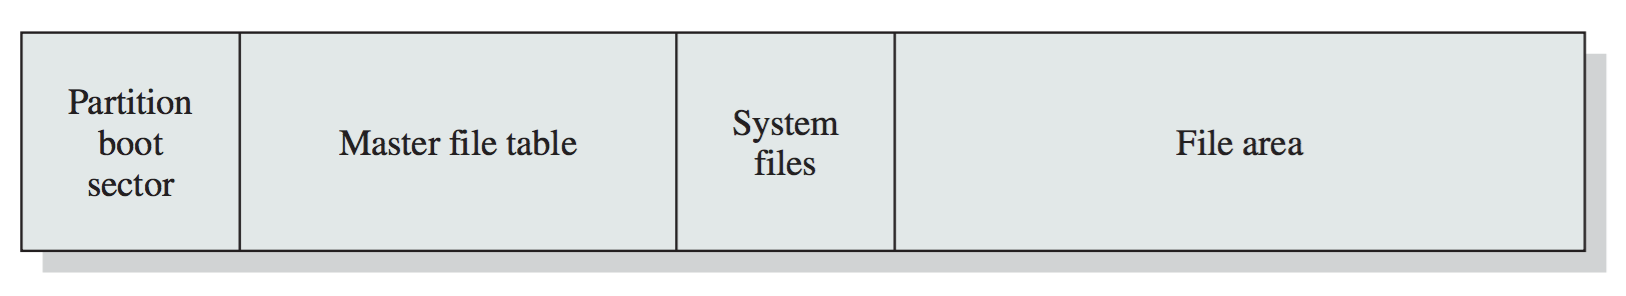
\includegraphics[width=0.6\textwidth]{images/ntfs-volume.png}\\
	Standard layout of an NTFS volume~\cite{osi}.
\end{center}

The Master File Table (MFT) contains information about all the files and folders. Following the that, a block is allocated to system files that contain some important system information~\cite{osi}:

\begin{enumerate}
	\item \textbf{MFT2}: Mirror of the first few rows of the MFT (in case the original is damaged).
	\item \textbf{Log File}: The journalling transaction log.
	\item \textbf{Cluster Bitmap}: Bitmap showing which of the clusters are in use.
	\item \textbf{Attribute Definition Table}: Attribute types supported on this volume.
\end{enumerate}

NTFS uses journalling to ensure that the file system will be in a consistent state at all times, even after a crash or restart. There is a service responsible for maintaining a log file that will be used to recover in the event that things go wrong.  Note that the goal of recovery is to make sure the system-maintained metadata is in a consistent state; user data can still get lost. This was a decision on the part of Microsoft to make the recovery operations significantly simpler and faster.

All metadata changes are written sequentially to a log file; once the changes are written to the log, control may return to the program that requested the operation. Meanwhile, the log entries are actually carried out. As changes are made, a pointer is updated to indicate which of the log entries have really happened and which have not. When an entire transaction is completed, it is removed from the log file. If the system crashes, the log file will contain zero or more transactions. If there are zero there is no problem: nothing was in progress at the time of the crash. If there are some, then the transactions were not completed and the operations should still be carried out. If a transaction was aborted (not committed), we walk backwards through the log entries to undo any completed operations and go back to the state before the start of the transaction~\cite{osc}.

Even though a particular write may not have taken place because of a crash, resulting in some data loss, at least the system will always remain in a consistent state. As a side benefit, we can sometimes re-order the writes to get better performance (e.g., schedule them in such a way that we get better disk utilization).


The actual implementation of journalling works as follows~\cite{russ}:

\begin{enumerate}
	\item Record the change(s) in the log file in the cache.
	\item Modify the volume in the cache.
	\item The cache manager flushes the log file to disk.
	\item Only after the log file is flushed to disk, the cache manager flushes the volume changes.
\end{enumerate}

What's really interesting about this is that the changes are carried out in the background, that is to say, asynchronously. A program can say that it wants to write some data, and not have to wait for the data to be written before going on to the next thing. How interesting! Can we get that behaviour in our (regular) program? Yes we can...

\bibliographystyle{alphaurl}
\bibliography{252}


\end{document}